% =============================================================================
% The CGAL User Manual
% Chapter: Geometric Optimisation
% Section: QP solver
% =============================================================================
\newcommand{\qprel}{\ccTexHtml{\gtreqless}{&nbsp;~&nbsp;}}

\ccUserChapter{QP\_solver}\label{QP_solver}
\ccChapterRelease{Release: WIP (\today)}
\ccChapterAuthor{Kaspar Fischer \and Bernd G{\"a}rtner 
\and Sven Sch{\"o}nherr \and Frans Wessendorp}

\section{Getting started}
This section explains what linear and quadratic programs are, gives a
simple example of a quadratic program, and shows how CGAL can be used
to solve it.

\subsection{What is a quadratic program?}
This package lets you solve \emph{convex quadratic programs} of the 
general form
\begin{eqnarray*}
\mbox{(QP)}&\mbox{minimize} & x^{T}Dx + c^{T}x + c_0 \\
&\mbox{subject to}   & Ax\qprel b, \\
&& l \leq x \leq u
\end{eqnarray*}
over $n$ variables $x=(x_0,\ldots,x_{n-1})$.

Here, $A \in \R^{m \times n}$ is the \emph{constraint matrix} and $b
\in \R^{m}$ the \emph{right-hand} side. The symbol ``$\qprel$'' in the
program's set $Ax \qprel b$ of $m$ \emph{constraints} indicates that for
$i=1,\ldots,m$, the $i$-th constraint may either be an inequality
$(Ax)_i \leq b_i$ or $(Ax)_i \geq b_i$, or an equality $(Ax)_i = b_i$.

Furthermore, $l\in
(\R\cup\{-\infty\})^n$ and $r\in (\R\cup\{\infty\})^n$ are \emph{bounds}
for the variables. Consequently, each
variable $x_j$, $j\in\{0,\ldots,n-1\}$, can be \emph{free} (if
$l_j=-\infty$ and $r_j=\infty$), \emph{upper-bounded} (if
$u_j\neq\infty$) and/or \emph{lower-bounded} (if
$l_j\neq-\infty)$.  

$D \in \R^{n \times n}$ is the \emph{quadratic
objective function matrix}. $D$ must be symmetric and 
positive-semidefinite in order for the \emph{quadratic objective function}
$x^{T}Dx$ to be convex. $c \in \R^{n}$ is the \emph{linear
objective function}, and $c_0$ is the \emph{constant term}. The full
\emph{objective function} is the sum of the quadratic, the linear, and
the constant term.

\emph{Solving} the quadratic program means to find a vector $x^*$ such
that $Ax^*\qprel b, l\leq x^*\leq u$ (a \emph{feasible solution}) with
the smallest objective function value among all feasible solutions.
Such a solution may not exist, see Sections
\ref{sec:QP-infeasible} and \ref{sec:QP-unbounded} below.

\subsection{Linear and nonnegative programs.}
If $D=0$, the quadratic program is in fact a \emph{linear program},
and in the case that $l$ is the zero vector and all entries of
$u$ are $\infty$, the program is said to be \emph{nonnegative}. The 
package offers dedicated solution methods for these special cases,
see Sections \ref{sec:QP-lp} and \ref{sec:QP-nonnegative} below.

\subsection{A first example}
Let's consider the following quadratic program in two variables:
\[
\begin{array}{lrcl}
\mbox{minimize}       & x^2 + 4(y-4)^2 &(=& x^2 + 4y^2 - 32y + 64) \\
\mbox{subject to}     & x + y &\leq& 7 \\
                      & -x + 2y &\leq& 4 \\
                      & x &\geq& 0 \\
                      & y &\geq& 0 \\
                      & y &\leq& 4
\end{array}
\]

Figure \ref{fig:QP-first_qp} shows a planar drawing of this. The figure
depicts the five inequalities of the program, along with the
\emph{feasible region} (green), the set of points that satisfy all the
five constraints. The dashed elliptic curves represent \emph{contour lines} 
of the objective function, i.e. along each dashed curve, the objective
function value is constant. 

The global minimum of the objective function is attained at 
the point $(0,4)$, and the minimum within the feasible region appears
at the point $(2,3)$ marked with a black dot. The value of the objective
function at this optimal solution is $2^2 + 4(3-4)^2 = 8$.

\begin{figure}[htbp]
\begin{ccTexOnly}
\begin{center}
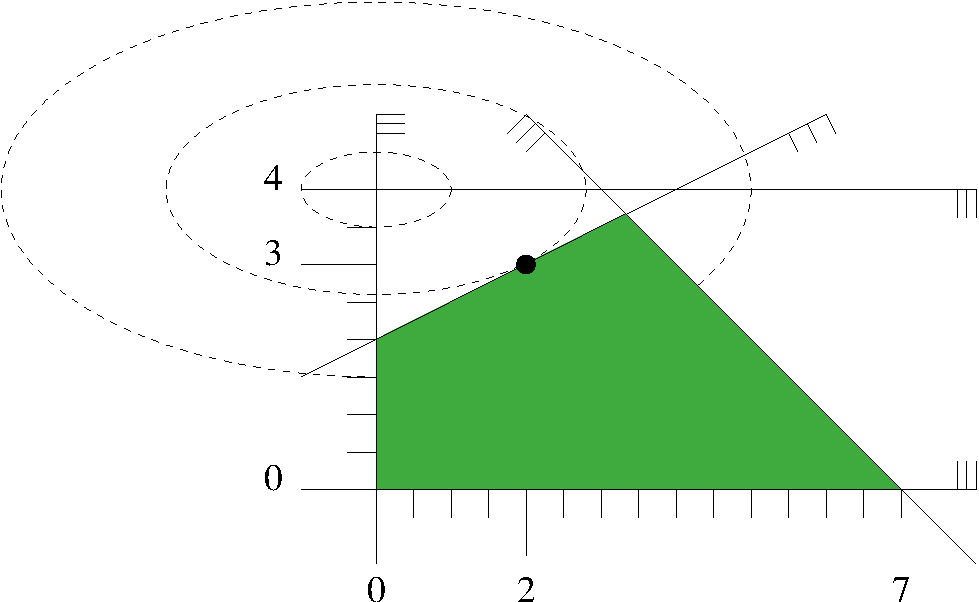
\includegraphics{QP_solver/first_qp} % omit suffix .eps to supprt PS and PDF
\end{center}
\end{ccTexOnly}
\caption{A quadratic program in two variables
\label{fig:QP-first_qp}}

\begin{ccHtmlOnly}
<CENTER>
<IMG BORDER=0 SRC="./first_qp.gif" ALIGN=center ALT="A quadratic program in two variables">
</CENTER>
\end{ccHtmlOnly}
\end{figure}

Here is how this quadratic program can be solved in CGAL.
The output will be:
\begin{verbatim}
Optimal feasible solution: 2/1  3/1
Optimal objective function value: 8/1
\end{verbatim}

\ccIncludeExampleCode{QP_solver/first_qp.cpp}


\section{Which problems can efficiently be solved?}

\section{Linear programs}\label{sec:QP-lp}

\section{Nonnegative programs}\label{sec:QP-nonnegative}

\section{The solution}

\section{Infeasibility}\label{sec:QP-infeasible}

\section{Unboundedness}\label{sec:QP-unbounded}

\section{The important variables}

\section{The important constraints}

\section{Certificates for the solution}



